\chapter{Introduction}
% \label{chap:intro}

% \section{Introduction}
\section{Motivations}
% \label{sec:motivation}

The process of web development has been significantly transformed by the introduction and adoption of frameworks. Frameworks have become the industry standard, providing developers with structured, reusable tools that simplify the creation of web applications. This evolution has also been greatly influenced by the rise of LLMs like OpenAI's Codex \cite{chen2021openai_codex}, Google's Gemini \cite{gemini}, and GitHub Copilot\footnote{Github Copilot - \url{https://copilot.github.com/}}, which have made coding more accessible by offering automated code generation, real-time suggestions, and debugging assistance. These tools have made entry into web development easier than ever, lowering barriers for beginners and speeding up development processes.

However, despite these advancements, LLMs still face certain limitations, such as hallucinations, difficulties in referencing external sources, and performance issues when handling specific tasks. A promising solution to mitigate these limitations is using RAG. RAG enhances the generative capabilities of LLMs by retrieving relevant external information before generating content, improving both the accuracy and relevance of the output. This technique is particularly beneficial in domains like web development, where staying up-to-date with framework versions and ensuring compatibility across services is critical. Incorporating RAG helps bridge the gap between rapidly evolving frameworks and the knowledge developers need to make informed decisions about the tools and technologies they use.

\begin{figure}[H]
\vspace{2pt}
\centering
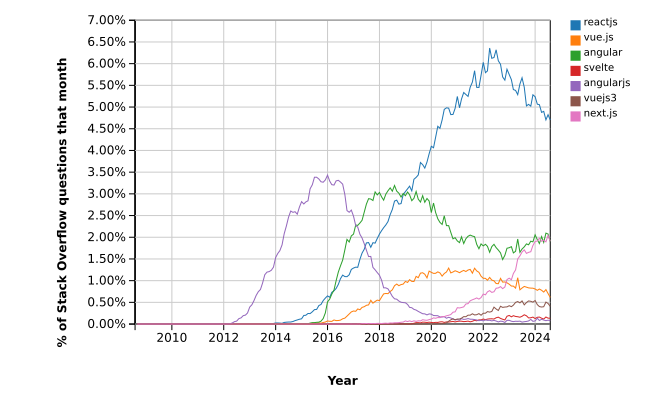
\includegraphics[width=1\textwidth]{Images/Introduction/stackoverflow-trends-chart.png}
\vspace{.1cm}
\caption{The popularity of frameworks based on StackOverflow questions 2008-2024}
\end{figure}

To illustrate, consider the Next.js framework, which has gained significant popularity in recent years. Built on top of React.js (currently the most popular front-end library), Next.js has seen rapid growth and frequent updates. For instance, version 13.0.0 of Next.js was released on October 25th, 2022, followed by multiple version 13.x.x updates, until version 14.0.0 was released on October 26th, 2023. Just 1 year later, they released version 15.0.0 for the framework with many breaking changes\footnote{\href{https://nextjs.org/blog}{The latest Next.js news - https://nextjs.org/blog}}. This rapid pace of development introduces challenges for developers who need to maintain or upgrade their codebases, especially considering that React.js itself has also undergone significant changes, such as the switch from version 18.0.0 to 19.0.0, which involved major updates\footnote{\href{https://react.dev/blog/2024/04/25/react-19-upgrade-guide}{How to Upgrade to React 18 - https://react.dev/blog/2024/04/25/react-19-upgrade-guide}}.

\section{Objectives}

The objective of this research is to develop a tool, specifically a VSCode extension, that facilitates the web development process by addressing common challenges associated with modern frameworks. The tool aims to:

\begin{itemize}
  \item Utilize RAG to assist developers with question answering, code generation, and code review. RAG will retrieve relevant information from documentation or community forums to enhance the accuracy and relevance of the tool's suggestions.
  \item Analyze the user's codebase and suggest modifications for parts that are no longer relevant, particularly when updating the code to newer versions of a framework.
\end{itemize}

This extension will help streamline the development process, making it easier for developers to maintain, upgrade, and enhance their applications with minimal friction.

\section{Scope}
The scope is intentionally confined to Next.js as the primary framework for web application development, enabling a focused exploration of its interaction with RAG methodologies. Additionally, the implementation targets applications written in JavaScript, TypeScript, HTML, and CSS, ensuring compatibility with commonly used web development programming languages.

% In this thesis, we aim to focus on the Next.js framework and the common packages that are often used alongside it, as well as Firebase for hosting purposes. The scope of the research includes the design and implementation of the RAG pipeline, the integration of the VSCode extension, and the evaluation of the system’s effectiveness in improving the development experience for Next.js applications.

% Specifically, our scope will only includes the technologies of Next.js - main framework used for the web application development.

% The tool will specifically target applications written in JavaScript, TypeScript, HTML, and CSS.
% Specifically, the scope includes the following technologies:

% \begin{itemize}
%   \item Next.js: The main framework used for web application development.
%   \item Firebase: Used for hosting Next.js applications and providing backend services.
%   \item Tailwind CSS: A utility-first CSS framework for designing responsive user interfaces.
%   \item Framer Motion: A popular library for animations and interactions.
%   \item Shadcn UI: A component library for UI elements.
%   \item Zod: A TypeScript-first schema declaration and validation library.
%   \item Prisma: An ORM for interacting with the database in a type-safe manner.
%   \item Firebase SDK: The official Firebase SDK is used for integration with Firebase services.
% \end{itemize}



% The focus will be on understanding how these tools and libraries can be used effectively in combination with Next.js and Firebase, with an emphasis on addressing issues related to rapid framework evolution and interoperability between services.

\section{Challenges}

Developing this tool involves several challenges:

\begin{itemize}
  \item Efficient Context Management: Since the goal is to make the tool lightweight, storing and managing the context of a user's codebase in a way that allows for fast retrieval without overwhelming system resources is a major challenge.
  \item Data Curation Complexity: The data curation process requires extensive knowledge about the framework.
  \item Handling Framework Updates: Keeping the tool updated with the frequent changes in frameworks like Next.js and their associated packages is challenging. Continuous updates are needed to ensure compatibility and provide accurate suggestions.
  \item User Experience: Balancing the amount of information presented to the user without overwhelming them is essential. The tool should provide meaningful insights and recommendations without causing information overload.
\end{itemize}

\section{Structure of the report}

\textbf{Chapter 1. Introduction.} 
This chapter introduces the motivations, objectives, and scope of the research. It highlights the challenges of web development and the role of RAG in enhancing efficiency and accuracy. The chapter outlines the structure of the report, providing a roadmap for the research presented.

\textbf{Chapter 2. Preliminaries.} 
This chapter provides foundational knowledge on RAG, emphasizing its retriever and generator components. It discusses indexing, vector embeddings, and augmentation methods, offering a clear understanding of the technologies used. Key concepts of the Next.js framework and associated development tools are also introduced.

\textbf{Chapter 3. Related Works and Tools.} 
This chapter explores prior research on RAG and its application in web development. It reviews developer tools such as VSCode extensions and discusses strategies for retrieval and augmentation. Comparative analyses of existing frameworks and methodologies are also presented.

\textbf{Chapter 4. Approach.} 
This chapter describes the proposed solution, including the architecture of the RAG-enhanced system. It explains the rationale for selecting specific models like BGE-M3 and Qwen and details the integration of local vector storage with the Next.js framework to ensure efficient retrieval and generation.

\textbf{Chapter 5. Initial implementation.} 
This chapter outlines the step-by-step development process of the RAG pipeline. It includes data preparation, database setup, and integration with the VSCode extension. Challenges encountered during implementation and their solutions are also discussed.

\textbf{Chapter 6. Evaluation plan.} 
This chapter evaluates the system using metrics such as accuracy and developer productivity. It describes the testing methodology, compares results with existing solutions, and highlights the strengths and limitations of the proposed approach.

\textbf{Chapter 7. Future plan.} 
The final chapter summarizes the contributions of the research and discusses potential areas for improvement. It offers recommendations for extending the system’s compatibility and incorporating advanced retrieval techniques to enhance performance and scalability.


% Background knowledge is then provided to explain the technologies and methodologies used. A review of related work follows, including research and existing solutions in web development, and Retrieval-Augmented Generation (RAG). The approach section describes the proposed solution, detailing the architecture and methodology for building the VSCode extension. The implementation section outlines the development process, and tools used. The evaluation presents the metrics, testing strategies, and results, along with comparisons to other solutions. Finally, the conclusion summarizes the achievements, discusses limitations, and offers suggestions for future improvements, with a reference section listing all the sources used.